\chapter{界面设计}
\section{客户端界面}
A. 对于用户注册与管理系统的用户接口说明如下,这一部分对应于功能需求中新用户注册、个人信息查询与修改、查询考试信息以及预缴费的部分:

\begin{figure}[ht]
\centering
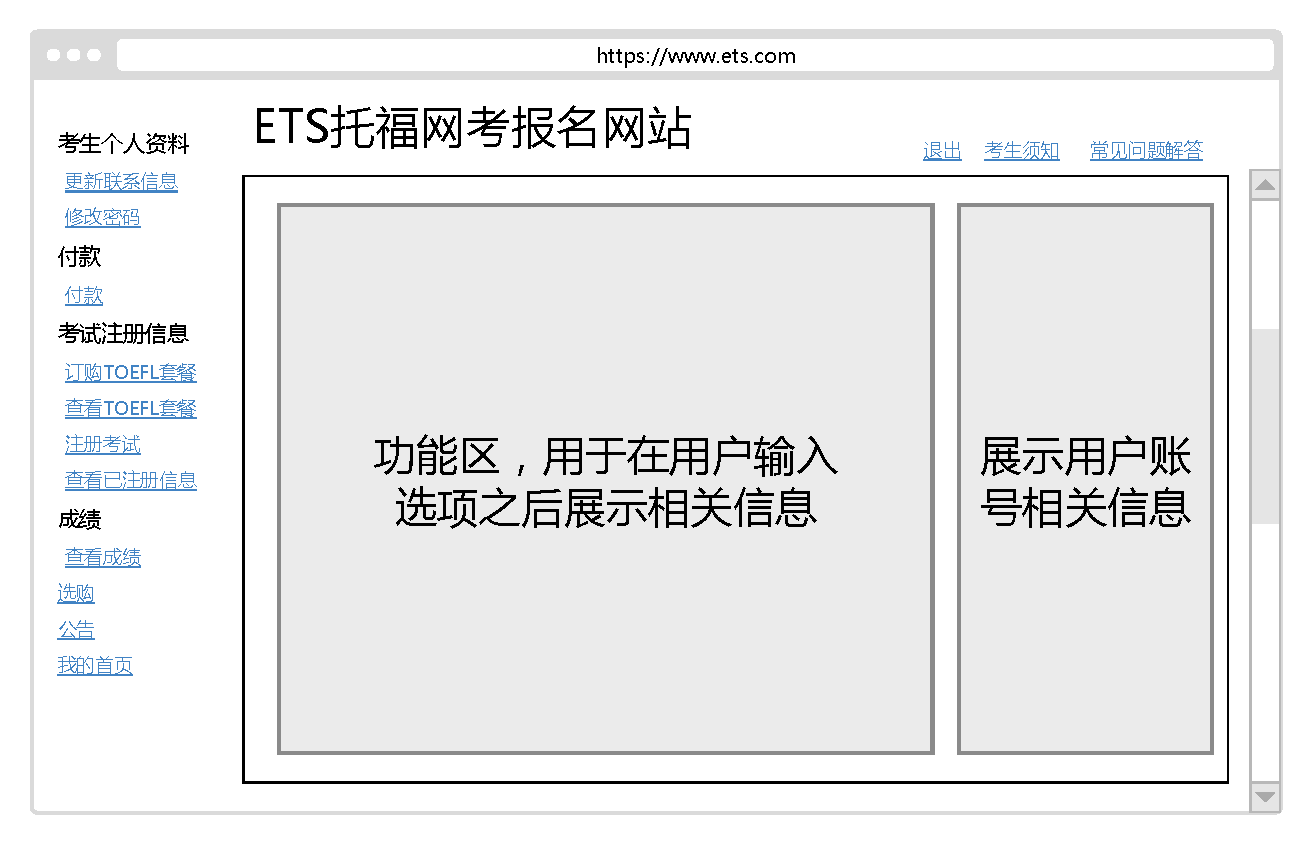
\includegraphics[width=10cm]{UI}
\caption{用户接口A}\label{fig:noted-figure}
%\note{the solid lines represent the time histogram of the spontaneous activities of an old monkey cell(gray) and a young monkey cell (black). The bin-width is 1}
\end{figure}

用户使用浏览器输入网址***.org后进入登录界面。输入ID和密码即可登录。在登录框下部提供两个按键“新用户注册”和“密码找回”。

用户点击“新用户注册”按键后,进入注册界面,其中包括各个文本框与下拉框供用户输入信息,所需输入的信息已在3.1节详细说明。

用户点击“密码找回”按键后,进入验证界面,可以选择邮箱验证或手机验证。通过注册时所填的邮箱或手机可以得到验证码,用户输入正确的验证码后,可以设置新密码。

当用户成功登录后,将进入个人中心界面,其中提供了各个功能板块,每个里面包括了一组相似功能的按键。

1、个人资料:提供“更新联系信息”和“修改密码”的按键;
	
2、考试记录:提供“考位查询”、“全年考试时间与地点查询”、“注册考试”、“查看已注册考试”、“查看成绩”的按键;

3、余额:提供“预付款”的按键。

\section{服务器端界面}
B. 对于试题管理系统的用户接口说明如下,这一部分对应于功能需求中题库维护、试题成型和试卷批改的部分:

\begin{figure}[ht]
\centering
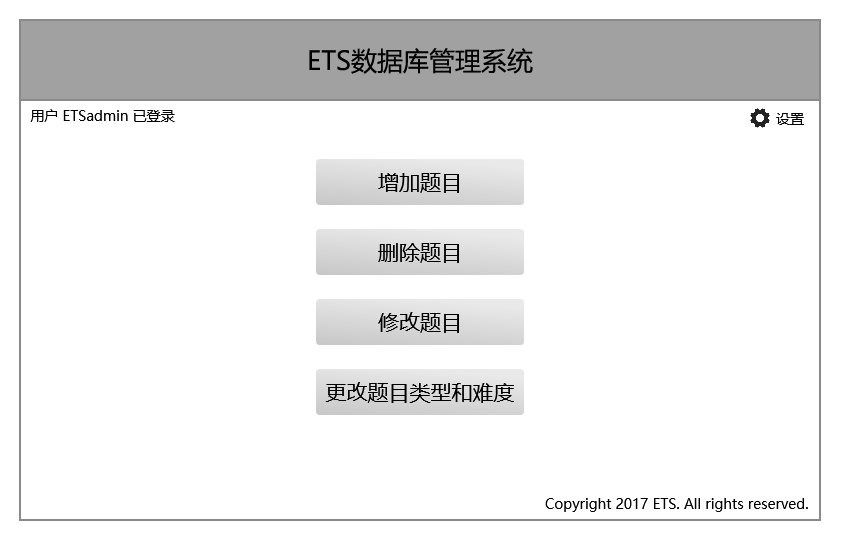
\includegraphics[width=10cm]{UI2.png}
\caption{用户接口B1}\label{fig:noted-figure}
%\note{the solid lines represent the time histogram of the spontaneous activities of an old monkey cell(gray) and a young monkey cell (black). The bin-width is 1}
\end{figure}

\begin{figure}[ht]
\centering
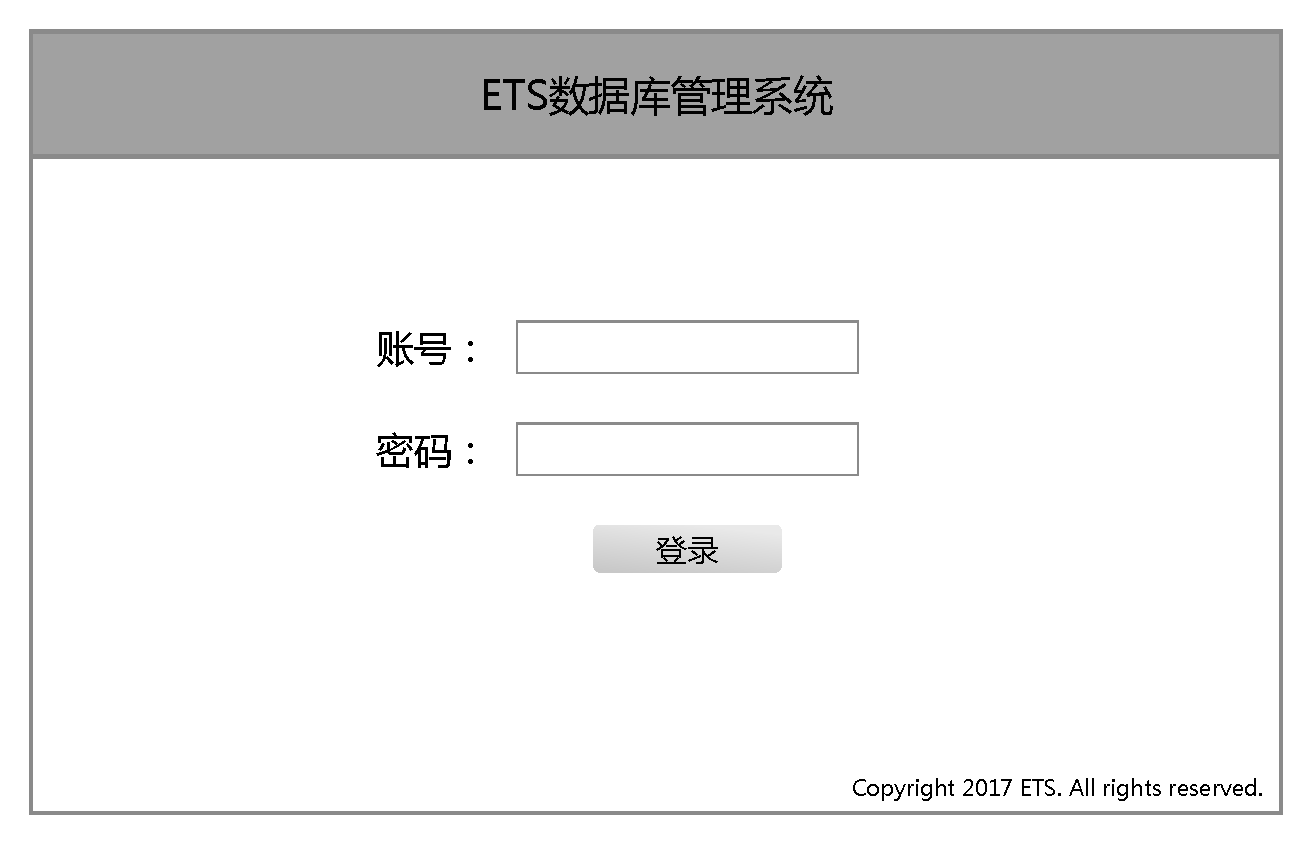
\includegraphics[width=10cm]{UI2-2}
\caption{用户接口B2}\label{fig:noted-figure}
%\note{the solid lines represent the time histogram of the spontaneous activities of an old monkey cell(gray) and a young monkey cell (black). The bin-width is 1}
\end{figure}

管理人员在服务器上运行指定的应用程序后进入登录界面,显示输入框要求输入账户和密码;登录成功后进入主界面,主界面的中央显示主菜单,菜单的选项同3.1中的说明相对应;右下角显示设置字样,点击后将能够查看设置并且进行修改。用户选择任意选项之后,主界面将按照3.1中的功能需求所对应的部分列出具体选项以及显示内容。

C. 对于考试系统的用户接口说明如下,这一部分对应于功能需求中试卷分发及测试的部分:

\begin{figure}[ht]
\centering
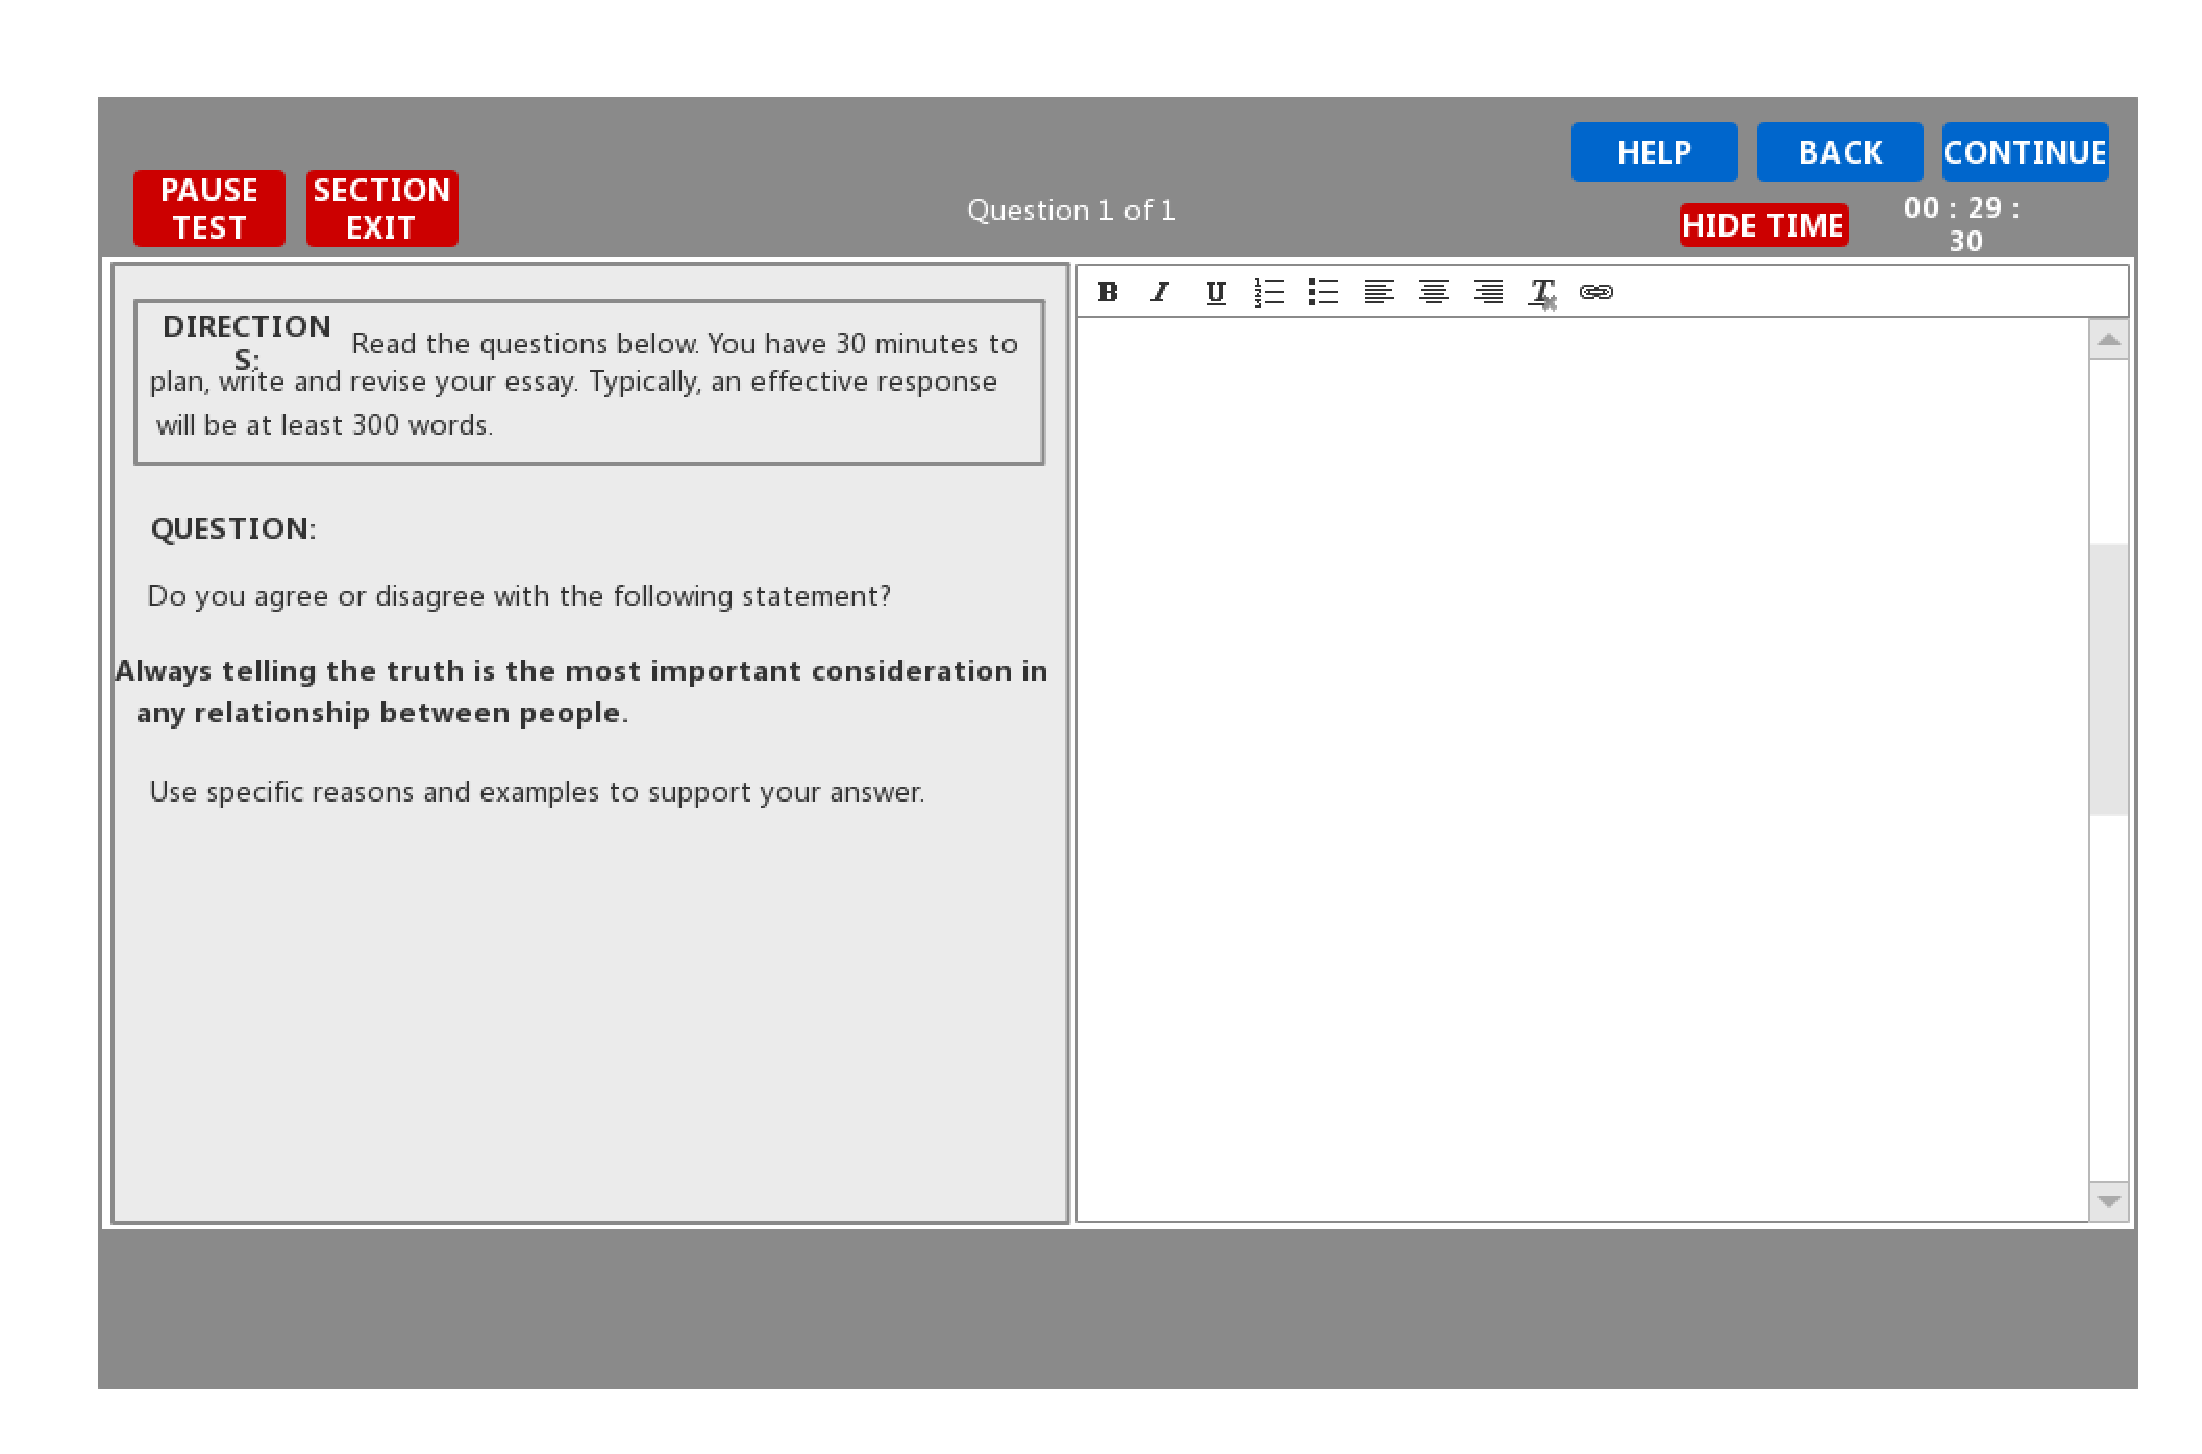
\includegraphics[width=15cm]{ETSwriting}
\caption{用户接口C1}\label{fig:noted-figure}
%\note{the solid lines represent the time histogram of the spontaneous activities of an old monkey cell(gray) and a young monkey cell (black). The bin-width is 1}
\end{figure}

\begin{figure}[ht]
\centering
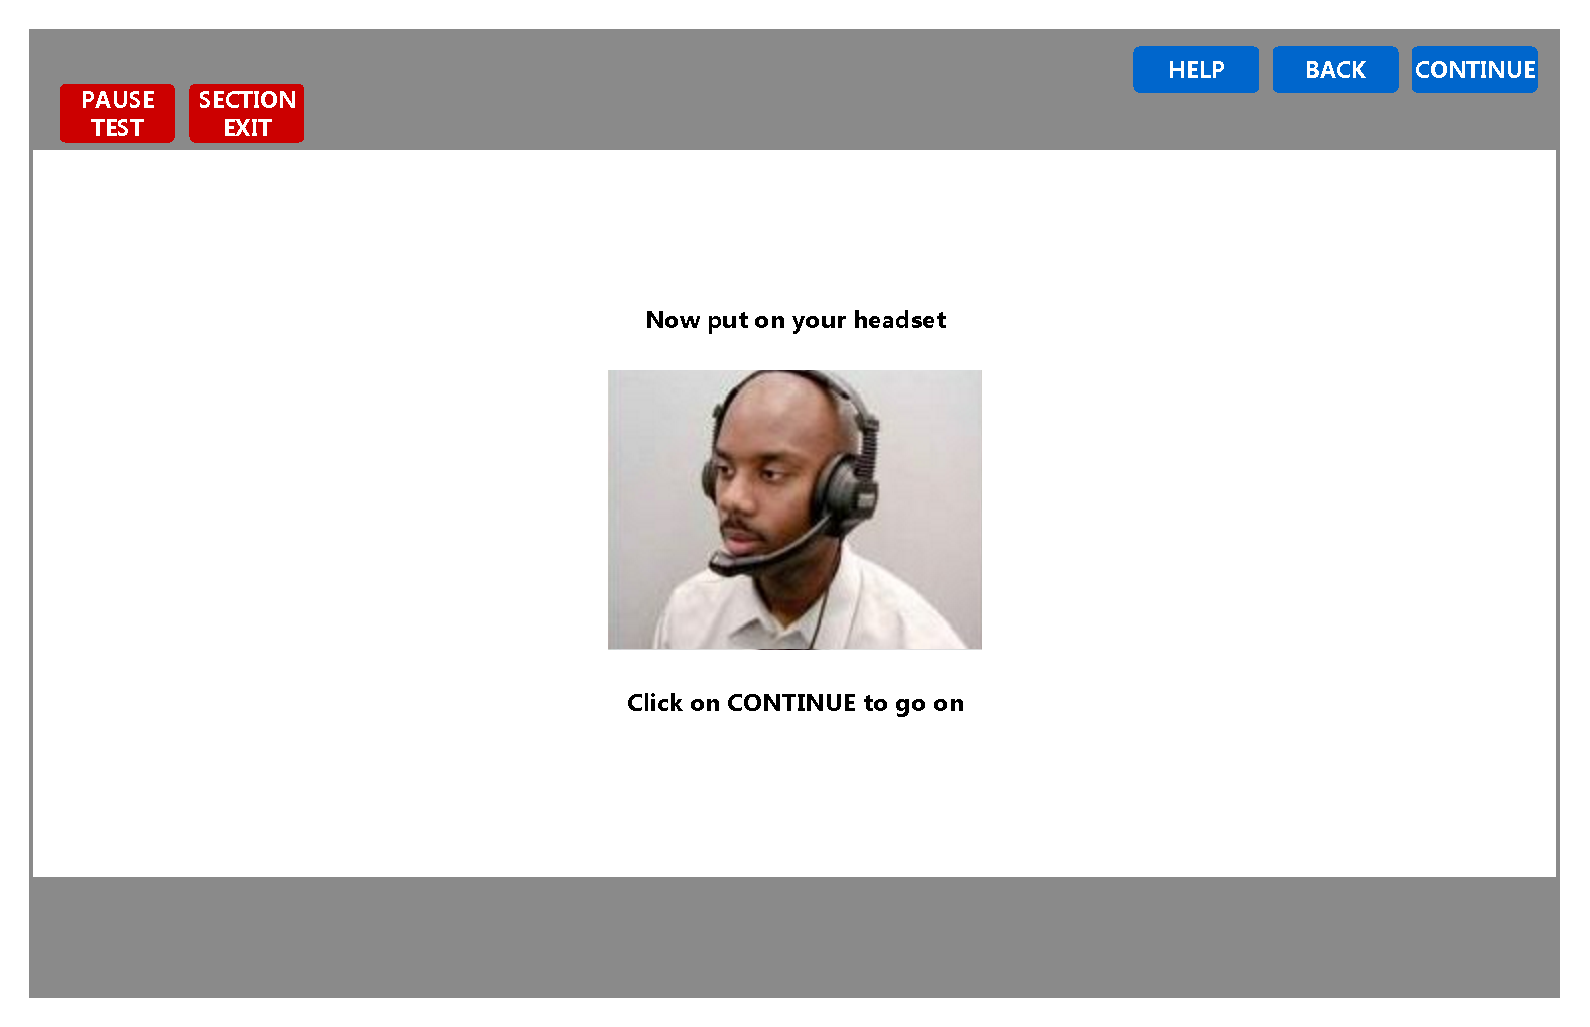
\includegraphics[width=15cm]{ETSlistening}
\caption{用户接口C2}\label{fig:noted-figure}
%\note{the solid lines represent the time histogram of the spontaneous activities of an old monkey cell(gray) and a young monkey cell (black). The bin-width is 1}
\end{figure}

用户将在考场给定的设备上使用本系统。考试未开始时,主界面将显示输入框,提示用户输入验证信息;

用户完成验证之后,主界面将显示用户的注册信息,直至考试开始;

考试开始之后,主界面将显示题目和对应的材料。用户能够根据鼠标点击来选择题目所对应的选项;主界面右上角提供调节音量、切换至下一题、切换回上一题、确认完成本部分的按钮,用户点击之后将触发相应的动作,该动作若当前不可触发应该显示为灰色;在按钮下方实时显示当前部分所剩余的时间,并且在时间的右侧显示“隐藏时间”的按钮,用户点击之后时间将被隐藏。

另外,在展示题目时,如果该部分材料需要和题目一同出现,那么将以页面的中轴线为界,在右侧显示材料,左侧显示相应的题目。对于阅读材料,用户应当能够利用鼠标滚轮上下移动材料。只显示题目时,题目应当显示在屏幕中央。

以上三部分都应具有友好的用户界面和使用提示,使得没有系统使用基础的用户不需要经过特定的培训就可以顺利使用本系统。
